\documentclass[11pt,a4paper]{article}
\usepackage[spanish,es-noshorthands,es-tabla]{babel}
\usepackage[utf8]{inputenc}
\usepackage[T1]{fontenc}
\usepackage{lmodern}
\usepackage{microtype}
\usepackage[margin=2.3cm]{geometry}
\usepackage{amsmath,amssymb,amsthm,bm}
\usepackage{graphicx}
\usepackage{booktabs,tabularx,multirow}
\usepackage{xcolor}
\usepackage{tikz}
\usetikzlibrary{positioning,arrows.meta,calc}
\usepackage{enumitem}
\usepackage{caption}
\usepackage[section]{placeins}
\usepackage[colorlinks=true,linkcolor=blue!50!black,citecolor=blue!50!black,urlcolor=blue!50!black]{hyperref}
\usepackage{algorithm}
\usepackage{algpseudocode}

\definecolor{azul}{HTML}{2A78D6}
\definecolor{naranjo}{HTML}{EB6834}
\definecolor{tinta}{HTML}{52514E}
\newtheorem{teorema}{Teorema}
\newtheorem{corolario}{Corolario}
\newtheorem{proposicion}{Proposición}
\theoremstyle{definition}
\newtheorem{definicion}{Definición}
\theoremstyle{remark}
\newtheorem*{obs}{Observación}
\newcommand{\E}{\mathbb{E}}
\newcommand{\ip}[1]{\left\langle #1 \right\rangle}
\renewcommand{\Re}{\operatorname{Re}}
\setlength{\parskip}{3pt}
\captionsetup{font=small,labelfont=bf}

\title{\textbf{Sinergia fraterna}\\[2pt]
\large Una métrica para localizar la banda de resonancia usando la estructura padre--hijos del árbol MDFD}
\author{Cristóbal Martínez Arochas\\
\small Detección de Anomalías en Sistemas Críticos --- Prof.\ Nibaldo Rodríguez A.\\
\small Ingeniería Civil en Ciencia de Datos, PUCV}
\date{Septiembre 2026}

\begin{document}
\maketitle

\begin{abstract}
El kurtogram diádico evalúa cada nodo del árbol MDFD por separado y elige $\arg\max K_{\ell,m}$. Así ignora lo único que el árbol aporta además de una grilla de bandas: la relación exacta entre un padre y sus dos hijos ($B_{\ell,m}=B_{\ell+1,2m}\,\dot\cup\,B_{\ell+1,2m+1}$). Aquí se demuestra una \emph{identidad de herencia}: la curtosis compleja de un padre es igual a la curtosis de sus hijos ponderada por energía más un término de interacción, la \textbf{sinergia fraterna} $S_{\ell,m}$, que mide cuánto se co-modulan las envolventes de los dos hermanos.
El ruido gaussiano en bandas disjuntas da $S\approx 0$. Un impacto que excita una resonancia modula ambos hijos a la vez y da $S>0$. De la identidad se deducen:
(i)~una explicación de por qué el kurtogram deriva hacia los niveles profundos;
(ii)~una métrica ciega nueva, estandarizada con surrogados que conservan a los hijos;
(iii)~una descomposición de $S$ en frecuencia cíclica, que da un espectro de envolvente cruzado entre hermanos insesgado frente al ruido.
Se valida con simulaciones de verdad conocida y con los registros CWRU a 12~kHz (DE y FE), con los mismos criterios de diagnóstico para todos los métodos.
\end{abstract}

\tableofcontents
\newpage

%==========================================================================
\section{Punto de partida: qué hace hoy el árbol MDFD}
%==========================================================================
Con la notación del curso, $X[k]=\mathrm{FFT}\{x[n]\}$ y, en el nivel $\ell$, la banda $m$ es
\[
B_{\ell,m}=[m\Delta f_\ell,(m+1)\Delta f_\ell),\qquad \Delta f_\ell=\frac{F_s}{2^{\ell+1}},\qquad x_{\ell,m}[n]=\mathrm{IFFT}\{H_{\ell,m}[k]X[k]\}.
\]
Para cada nodo se forma la señal analítica centrada $\tilde z_{\ell,m}=z_{\ell,m}-\overline{z_{\ell,m}}$ y la curtosis compleja
\[
K_{\ell,m}=\frac{\hat\mu_{4,\ell,m}}{\hat\mu_{2,\ell,m}^2}-2,\qquad \hat\mu_{p}=\frac1N\sum_n|\tilde z[n]|^p .
\]
La banda elegida es $(\ell^\star,m^\star)=\arg\max K_{\ell,m}$. Las diapositivas ya señalan dos propiedades del árbol: los hijos parten exactamente al padre y los nodos de un mismo nivel son ortogonales. Sin embargo, el criterio de selección no usa ninguna de las dos. \textbf{La pregunta del profesor es justamente esa: ¿qué métrica aprovecha la estructura del árbol?}

%==========================================================================
\section{Lluvia de ideas: métricas que sólo existen porque hay un árbol}
%==========================================================================
La regla que usé para generar ideas: una métrica ``de árbol'' debe usar una relación entre nodos (padre--hijo, hermano--hermano, camino raíz--hoja o vecinos que cruzan una frontera). No basta con un valor por nodo. La Tabla~\ref{tab:ideas} resume las candidatas. Las tres primeras se desarrollan e implementan en este informe.

\begin{table}[!htb]
\centering\small
\begin{tabularx}{\textwidth}{@{}p{0.3cm}p{3.6cm}Xp{2.1cm}@{}}
\toprule
\# & Idea & Relación del árbol que explota / intuición física & Estado \\
\midrule
1 & \textbf{Sinergia fraterna $S$} & Padre $=$ hijo izq.\ $+$ hijo der. La curtosis del padre se descompone de forma exacta en herencia $+$ interacción. Un impacto resonante co-modula a ambos hermanos; el ruido no. & Desarrollada (§\ref{sec:teoria}) \\
2 & \textbf{Espectro de sinergia $s(\alpha)$} & La parte de co-modulación de $S$ es la integral del espectro cruzado entre las envolvente cuadráticas de los hermanos. Es un ``segundo sensor'' virtual: el ruido tiene media cero. & Desarrollada (§\ref{sec:ciclica}) \\
3 & \textbf{$Z$ por surrogados fraternos} & Desplazar circularmente un hijo conserva su espectro, su curtosis y la ortogonalidad, y destruye sólo la sincronía entre hermanos. Da una hipótesis nula exacta ``hijos independientes''. & Desarrollada \\
4 & Descenso por sinergia & Búsqueda raíz$\to$hoja con $O(L)$ decisiones, como un árbol de decisión: se baja mientras la curtosis sea ``heredada'' y se detiene cuando es ``sinérgica''. & Prototipo \\
5 & Persistencia de linaje & La firma cíclica de la falla debe heredarse a lo largo del camino raíz$\to$hoja. La resonancia está donde la tasa de herencia $\mathrm{SES}_{\text{hijo}}(f_d)/\mathrm{SES}_{\text{padre}}(f_d)$ cae bruscamente. & Idea \\
6 & Sinergia entre primos & Nodos adyacentes que \emph{no} son hermanos, $(\ell,2k{+}1)$ y $(\ell,2k{+}2)$, comparten una frontera heredada. Su co-modulación detecta resonancias partidas por fronteras de niveles superiores. & Idea \\
7 & Cascada de impulsividad & $D_{\ell,m}=\max_c w_c^2K_c/K_{\ell,m}$ dice de qué hijo proviene la impulsividad. Dibuja un grafo de flujo de $K$ por el árbol. & Idea \\
8 & Coherencia de fase entre hermanos & El término $S_{\text{fase}}$ de la identidad mide acoplamiento de fase a través de la frontera. Un impulso tiene fase lineal (retardo de grupo común); el ruido no. & Idea (término ya calculado) \\
9 & Ganancia de negentropía por división & Análogo al criterio de CART: $\Delta J=J(\text{padre})-\sum_c w_cJ(c)$, con $J$ la negentropía de la envolvente cuadrática. & Idea \\
10 & Sinergia cíclica ciega & Buscar $\alpha_0$ que maximice la sinergia neta en un peine armónico sin conocer $f_d$. Estima la frecuencia de falla y rechaza impulsos aleatorios. & Idea \\
\bottomrule
\end{tabularx}
\caption{Lluvia de ideas. ``Desarrollada'' significa teoría, código y validación en este documento.}
\label{tab:ideas}
\end{table}

%==========================================================================
\section{Teoría: la identidad de herencia de la curtosis}\label{sec:teoria}
%==========================================================================
Sea $p=(\ell,m)$ un nodo con hijos $a=(\ell+1,2m)$ y $b=(\ell+1,2m+1)$. Se escribe $z_p,z_a,z_b$ para sus señales analíticas centradas, $P_\bullet=\ip{|z_\bullet|^2}$ para las potencias ($\ip{\cdot}$ es el promedio temporal) y $w_a=P_a/P_p$, $w_b=P_b/P_p$.

\begin{proposicion}[El padre es la suma de sus hijos]\label{prop:suma}
$z_p[n]=z_a[n]+z_b[n]$ para todo $n$, $\ip{z_az_b^*}=0$ y $P_p=P_a+P_b$ (es decir, $w_a+w_b=1$).
\end{proposicion}
\begin{proof}
El espectro analítico del nodo es $h[k]H_{\ell,m}[k]X[k]$, con $h=2$ en frecuencias positivas. Esta operación es lineal en la máscara y $H_{\ell,m}=H_{a}+H_{b}$ porque los soportes son disjuntos. La IFFT es lineal, así que $z_p=z_a+z_b$. El centrado también es lineal. Por Parseval, $\ip{z_az_b^*}=\frac1{N^2}\sum_k Z_a[k]Z_b^*[k]=0$ porque los soportes no se tocan. La media sólo es no nula en el nodo que contiene $k=0$, que nunca es un hijo derecho, así que el centrado no rompe la ortogonalidad. Luego $|z_p|^2=|z_a|^2+|z_b|^2+2\Re(z_az_b^*)$ y, promediando, $P_p=P_a+P_b$.
\end{proof}

\begin{teorema}[Herencia de curtosis]\label{teo:herencia}
Para todo nodo padre se cumple, \textbf{exactamente} (sin aproximaciones):
\begin{equation}\label{eq:herencia}
\boxed{\;K_p \;=\; \underbrace{w_a^2K_a+w_b^2K_b}_{\text{curtosis heredada}}\;+\;\underbrace{S_p}_{\text{sinergia fraterna}}\;}
\end{equation}
donde
\begin{align}
S_p &= S^{\mathrm{cov}}_p+S^{\mathrm{fase}}_p,\\
S^{\mathrm{cov}}_p &= \frac{4\,\mathrm{cov}\!\left(|z_a|^2,|z_b|^2\right)}{P_p^2}
      \qquad\text{(co-modulación de las envolventes)},\label{eq:scov}\\
S^{\mathrm{fase}}_p &= \frac{2\Re\ip{z_a^2\,z_b^{*2}}+4\ip{\left(|z_a|^2+|z_b|^2\right)\Re(z_az_b^*)}}{P_p^2}
      \qquad\text{(acoplamiento de fase)}.\label{eq:sfase}
\end{align}
\end{teorema}
\begin{proof}
Sea $c=z_az_b^*$. Elevando al cuadrado $|z_p|^2=|z_a|^2+|z_b|^2+2\Re c$:
\[
|z_p|^4=(|z_a|^2+|z_b|^2)^2+4(|z_a|^2+|z_b|^2)\Re c+4(\Re c)^2 .
\]
Como $(\Re c)^2=\tfrac12\left(|c|^2+\Re c^2\right)=\tfrac12\left(|z_a|^2|z_b|^2+\Re(z_a^2z_b^{*2})\right)$, al promediar se obtiene
\[
\ip{|z_p|^4}=\ip{|z_a|^4}+\ip{|z_b|^4}+4\ip{|z_a|^2|z_b|^2}+2\Re\ip{z_a^2z_b^{*2}}+4\ip{(|z_a|^2+|z_b|^2)\Re c}.
\]
Se escribe $\ip{|z_a|^2|z_b|^2}=\mathrm{cov}(|z_a|^2,|z_b|^2)+P_aP_b$, se divide por $P_p^2$ y se usa $\ip{|z_\bullet|^4}=(K_\bullet+2)P_\bullet^2$:
\[
K_p+2=w_a^2(K_a+2)+w_b^2(K_b+2)+4w_aw_b+S_p .
\]
Como $2w_a^2+2w_b^2+4w_aw_b=2(w_a+w_b)^2=2$, se obtiene \eqref{eq:herencia}.
\end{proof}

\noindent\textbf{Verificación numérica.} En el código, $|K_p-(w_a^2K_a+w_b^2K_b+S_p)|\approx10^{-15}$ (precisión de máquina) en los 63 nodos padre del árbol ($L=6$). Además, $\max|z_p-(z_a+z_b)|/\max|z_p|\approx6\times10^{-16}$.

\begin{figure}[!htb]
\centering
\begin{tikzpicture}[node distance=1.0cm and 2.2cm, every node/.style={font=\small},
  caja/.style={draw=tinta,rounded corners=3pt,minimum width=3.3cm,minimum height=0.9cm,align=center,fill=white}]
\node[caja,fill=azul!8] (p) {padre $B_{\ell,m}$\\ $K_p=w_a^2K_a+w_b^2K_b+\color{azul}S_p$};
\node[caja,below left=1.1cm and 0.1cm of p] (a) {hijo $B_{\ell+1,2m}$\\ $w_a,\;K_a$};
\node[caja,below right=1.1cm and 0.1cm of p] (b) {hijo $B_{\ell+1,2m+1}$\\ $w_b,\;K_b$};
\draw[-{Latex[length=2mm]},tinta] (p) -- (a);
\draw[-{Latex[length=2mm]},tinta] (p) -- (b);
\draw[azul,very thick,{Latex[length=2mm]}-{Latex[length=2mm]}] (a.east) -- node[below=2pt,align=center,text=azul]{\footnotesize co-modulación de envolventes\\\footnotesize $\mathrm{cov}(|z_a|^2,|z_b|^2)$} (b.west);
\end{tikzpicture}
\caption{La identidad de herencia. Lo que el padre ``tiene de más'' respecto de sus hijos es la sinergia $S_p$, que depende sólo de la \emph{interacción} entre los dos hermanos.}
\label{fig:diagrama}
\end{figure}

\subsection{Consecuencias}

\begin{corolario}[La sinergia es necesaria para que un padre le gane a sus hijos]\label{cor:sesgo}
Si $K_a,K_b\ge0$, entonces
\[
K_p>\max(K_a,K_b)\quad\Longrightarrow\quad S_p>\max(K_a,K_b)-(w_a^2K_a+w_b^2K_b)\;\ge\;\big(1-w_a^2-w_b^2\big)\max(K_a,K_b)\;\ge 0 .
\]
\end{corolario}
\begin{proof}
Se tiene $w_a^2K_a+w_b^2K_b\le(w_a^2+w_b^2)\max(K_a,K_b)$ y $w_a^2+w_b^2\le 1$.
\end{proof}
\noindent\emph{Lectura:} sin co-modulación entre hermanos, la curtosis \textbf{se diluye} al subir por el árbol, porque el padre mezcla energías con pesos $w^2<w$. El $\arg\max K$ solo puede quedarse en un nodo ancho si ahí hay sinergia real. Cuando no la hay, el máximo resbala hacia las hojas.

\begin{proposicion}[Por qué resbala: varianza del estimador por nivel]\label{prop:var}
Para ruido gaussiano complejo circular, $\operatorname{sd}(\hat K_{\ell,m})\approx 2/\sqrt{N_{\text{ef}}}$ con $N_{\text{ef}}\approx N/2^\ell$. Esto sale del método delta con $|z|^2\sim\mathrm{Exp}$: $\mathrm{Var}(\hat\mu_4/\hat\mu_2^2)\approx 4/N_{\text{ef}}$. Es decir, el ruido de estimación \emph{crece} como $2^{\ell/2}$.
\end{proposicion}
\noindent Una simulación Monte Carlo ($N=2^{14}$, 150 réplicas de ruido blanco) confirma que la desviación estándar crece como $2^{\ell/2}$, de 0{,}019 en $\ell=0$ a 0{,}096 en $\ell=5$ (la predicción es 0{,}016--0{,}088). En el nivel más profundo, con 64 nodos puramente ruidosos, el máximo esperado de $\hat K$ es cerca de $2{,}4\,\operatorname{sd}$, suficiente para ganarle a una resonancia débil. \textbf{El Corolario~\ref{cor:sesgo} y la Proposición~\ref{prop:var} juntos explican el sesgo del kurtogram hacia niveles profundos}, que en los experimentos (§\ref{sec:resultados}) es su principal modo de falla.

\begin{proposicion}[Nulidad bajo independencia]\label{prop:nula}
Si $z_a$ y $z_b$ son independientes y al menos uno es circular de media cero ($\E z=\E z^2=0$), entonces $\E[S_p]=0$.
\end{proposicion}
\begin{proof}
$\mathrm{cov}(|z_a|^2,|z_b|^2)=0$ por independencia. Además, $\E[z_a^2z_b^{*2}]=\E[z_a^2]\E[z_b^{*2}]=0$ y $\E[|z_a|^2z_az_b^*]=\E[|z_a|^2z_a]\E[z_b^*]=0$.
\end{proof}
\noindent El ruido gaussiano estacionario tiene coeficientes de Fourier (asintóticamente) independientes en bandas disjuntas, así que $S\approx0$. En la simulación con ruido blanco, la media de $\hat S$ es $|\bar S|<0{,}004$ en todos los niveles.

\subsection{Interpretación física}
\begin{table}[!htb]
\centering\small
\begin{tabularx}{\textwidth}{@{}p{4.3cm}p{2.3cm}X@{}}
\toprule
Contenido de los hijos & $S_p$ & Motivo \\
\midrule
Ruido gaussiano & $\approx0$ & Envolventes independientes (Prop.~\ref{prop:nula}). \\
Tonos (armónicos de giro, línea) & $\approx0$ & Envolvente constante, no hay modulación que compartir. \\
Impulso sólo en un hijo (resonancia angosta) & $\approx0$ & $K_a$ es alto pero no hay co-modulación: la curtosis es \emph{heredada} y conviene bajar al hijo. \\
Resonancia excitada por impactos que ocupa ambos hijos & $\gg0$ & Cada impacto enciende las dos sub-bandas al mismo tiempo: la banda es ``indivisible''. \\
Impactos aleatorios de banda ancha (EMI impulsiva) & $>0$ & También co-modulan. Una métrica ciega no puede distinguirlos (hace falta la versión cíclica, §\ref{sec:ciclica}). \\
Holgura (impactos a $k f_r$) & $>0$ & Co-modulan a $f_r$. Se separan con la versión cíclica dirigida a $f_d$. \\
\bottomrule
\end{tabularx}
\caption{Qué ve la sinergia.}
\end{table}

\subsection{Estandarización con surrogados fraternos}
El valor de $\hat S$ depende del nivel (Prop.~\ref{prop:var}) y de la forma de las distribuciones de los hijos. Para compararlo entre niveles se construye una hipótesis nula \emph{exacta} que conserva todo menos la interacción: se reemplaza $z_b[n]$ por $z_b[n-\tau]$ (desplazamiento circular con $\tau$ aleatorio). El desplazamiento no cambia $|Z_b[k]|$, así que conserva $P_b$, $K_b$ y la ortogonalidad con $z_a$. Por el Teorema~\ref{teo:herencia}, el padre surrogado cumple
\[
K_p^{\text{surr}}=w_a^2K_a+w_b^2K_b+S_p^{\text{surr}} .
\]
Con $R$ desplazamientos ($R=12$--$16$, con $|\tau|$ mayor que 4 tiempos de correlación del hijo) se define
\begin{equation}\label{eq:Z}
Z_{\ell,m}=\frac{S_{\ell,m}-\overline{S^{\text{surr}}_{\ell,m}}}{\operatorname{sd}\big(S^{\text{surr}}_{\ell,m}\big)} .
\end{equation}
$Z$ responde a una pregunta precisa: \emph{¿cuántas desviaciones estándar más impulsivo es el padre de lo que sería si sus dos hijos fueran independientes?} Es adimensional y comparable entre niveles.

\subsection{Algoritmos}
\begin{algorithm}[h]
\caption{Sinergograma (métrica ciega)}
\begin{algorithmic}[1]
\State $X\gets\mathrm{FFT}(x)$; obtener $z_{\ell,m}$ para $\ell=0,\dots,L$ (una IFFT por nodo, igual que el kurtogram)
\For{cada padre $(\ell,m)$, $\ell<L$}
  \State $a\gets(\ell{+}1,2m)$, $b\gets(\ell{+}1,2m{+}1)$; calcular $w_a,w_b,K_a,K_b$ y $S_{\ell,m}$ con \eqref{eq:scov}--\eqref{eq:sfase}
  \For{$r=1,\dots,R$} \State $S^{(r)}\gets S\big(z_a,\;\mathrm{roll}(z_b,\tau_r)\big)$ \EndFor
  \State $Z_{\ell,m}\gets\big(S_{\ell,m}-\mathrm{media}(S^{(r)})\big)/\mathrm{sd}(S^{(r)})$
\EndFor
\State \Return $(\ell^\star,m^\star)=\arg\max Z_{\ell,m}$ y el mapa $\{(f^c_{\ell,m},\Delta f_\ell,Z_{\ell,m})\}$
\end{algorithmic}
\end{algorithm}

\noindent\textbf{Descenso por sinergia} (variante $O(L)$). Se parte de la raíz. Si $Z_p\ge z_{\text{umbral}}$ (se usó 3) y $\ell>0$, la banda es indivisible y se detiene. Si no, se baja al hijo $c$ con mayor aporte heredado $w_c^2K_c$. Es la versión ``árbol de decisión'' de la identidad: el costo de dividir es perder la sinergia.

%==========================================================================
\section{Extensión cíclica: el espectro de sinergia}\label{sec:ciclica}
%==========================================================================
Por Wiener--Khinchin, la covarianza a retardo cero es la integral del espectro cruzado. Con $e_\bullet=|z_\bullet|^2-P_\bullet$ y $C_{ab}(\alpha)=\mathrm{CSD}(e_a,e_b)$:
\begin{equation}\label{eq:sespectro}
S^{\mathrm{cov}}_p=\int s_p(\alpha)\,d\alpha,\qquad s_p(\alpha)=\frac{4\,\Re\,C_{ab}(\alpha)}{P_p^2}.
\end{equation}
\textbf{La sinergia se descompone en frecuencias cíclicas.} Esto une la impulsividad (curtosis) con la cicloestacionariedad (espectro de envolvente) en un solo objeto. En el código, $\sum_\alpha\Re C_{ab}\Delta\alpha$ reproduce $\mathrm{cov}(|z_a|^2,|z_b|^2)$ con un error de $1{,}3\%$ (estimación de Welch).

\begin{proposicion}[El espectro de sinergia es insesgado frente al ruido]\label{prop:insesgo}
Sea $z_\bullet=s_\bullet+n_\bullet$ (falla $+$ ruido), con $n_a,n_b$ independientes entre sí y de la señal, circulares y de media cero. Entonces $\E[C_{ab}(\alpha)]=C_{|s_a|^2,|s_b|^2}(\alpha)$.
\end{proposicion}
\begin{proof}
$|z_a|^2=|s_a|^2+|n_a|^2+2\Re(s_an_a^*)$, y lo mismo para $b$. Todos los productos cruzados que involucran $n$ tienen esperanza nula: $|n_a|^2$ con $|n_b|^2$ por independencia (la media se quitó al centrar), términos con un solo factor $n$ por media cero, y $\Re(s_an_a^*)\Re(s_bn_b^*)$ porque $\E[n_an_b^*]=0$.
\end{proof}
\noindent En cambio, el SES clásico de un nodo acumula $S_{|n|^2}(\alpha)>0$, un piso de ruido positivo. El espectro cruzado entre hermanos se comporta como tener \emph{dos sensores} con ruidos independientes, pero con un solo acelerómetro: el árbol fabrica el segundo sensor. El ruido sólo aporta varianza, que baja como $1/\sqrt{\#\text{segmentos}}$ (Fig.~\ref{fig:ses}).

\paragraph{Sinergia dirigida.} Si $f_d$ es conocida (BPFO, BPFI o $2\,$BSF),
\[
S_p(f_d)=\sum_{h=1}^{3}\int_{|\alpha-hf_d|\le 0.02hf_d}\Big(s_p(\alpha)-\operatorname{mediana}_{\text{fondo local}}\,s_p\Big)\,d\alpha ,
\]
que se lee como la \emph{parte de la curtosis del padre explicada por la co-modulación de los hijos a la frecuencia de falla}. Se descuenta el fondo cíclico local, para no premiar la co-modulación de banda ancha de impulsos aleatorios. También se probó la \emph{coherencia fraterna} $\rho(\alpha)=\Re C_{ab}/\sqrt{S_{aa}S_{bb}}\in[-1,1]$.

\begin{figure}[!htb]
\centering
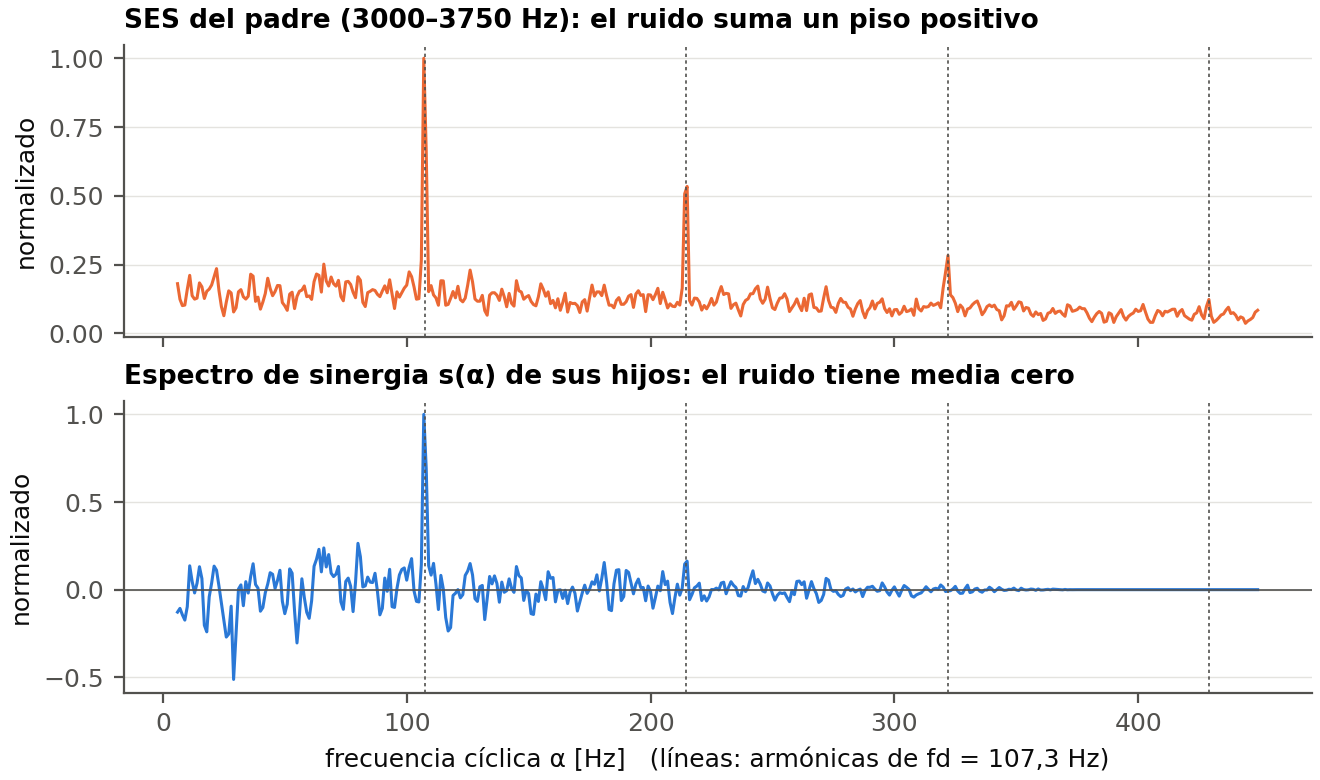
\includegraphics[width=0.86\textwidth]{../fig/ses_vs_sinergia.png}
\caption{Simulación a SNR $-16$~dB. Arriba: SES del nodo $(3,4)$, con piso positivo de ruido. Abajo: espectro de sinergia de sus dos hijos, donde el ruido oscila alrededor de cero y sobrevive la línea en $f_d$. Las armónicas superiores se atenúan porque la envolvente de cada hijo (375~Hz de ancho) tiene poco contenido sobre $\sim$300~Hz.}
\label{fig:ses}
\end{figure}

%==========================================================================
\section{Resultados}\label{sec:resultados}
%==========================================================================
\subsection{Diseño experimental}
\begin{itemize}[leftmargin=*,itemsep=1pt]
\item \textbf{Árbol:} MDFD con máscaras ideales en FFT, $F_s=12$~kHz y $L=6$ (hojas de 93{,}75~Hz). Es la misma implementación del curso.
\item \textbf{Criterio de diagnóstico, idéntico para todos los métodos:} en el SES de la banda elegida, la relación armónica/fondo en $f_d\pm2\%$ debe ser $\ge 6$~dB. El fondo es la mediana del SES en $f_d\pm0{,}3f_d$, sin contar el pico.
\item \textbf{Simulación:} falla de pista externa, $f_d=107{,}3$~Hz, con 1\% de deslizamiento aleatorio. Cada impacto excita una resonancia de $f_n=3{,}5$~kHz y $\zeta=0{,}04$. Hay 10~s de señal más ruido gaussiano (el SNR se mide sobre la potencia total de la falla). Escenarios:
A)~base;
B)~$+$~impactos aleatorios (Poisson, 3/s) en otra resonancia de 1{,}2~kHz;
C)~$+$~holgura: impactos a $f_r$ en 5{,}2~kHz;
D)~$+$~EMI (40 armónicos de 60~Hz) y tonos de giro/engrane;
E)~resonancia en 3~kHz, que cae sobre una frontera diádica en \emph{todos} los niveles.
Se hicieron 8 réplicas por celda.
\item \textbf{CWRU:} los 105 registros con falla a 12~kHz (60 DE y 45 FE). $f_d$ es BPFI, BPFO o $2\,$BSF, igual que en la clase para el registro 282. Para medir falsas alarmas de forma justa, cada registro también se evalúa en dos \emph{frecuencias señuelo} ($2{,}68f_r$ y $3{,}79f_r$ en DE; $2{,}47f_r$ y $5{,}47f_r$ en FE). Estas frecuencias están elegidas lejos de toda línea cinemática conocida (armónicos de $f_r$, BPFI, BPFO, BSF, $2\,$BSF, FTF y bandas laterales). Un método útil debe detectar en $f_d$ y \emph{no} en los señuelos. Se reporta $J=\text{TPR}-\text{FPR}$ (índice de Youden).
\end{itemize}

\subsection{Mapas: qué ve cada métrica}
\begin{figure}[!htb]
\centering
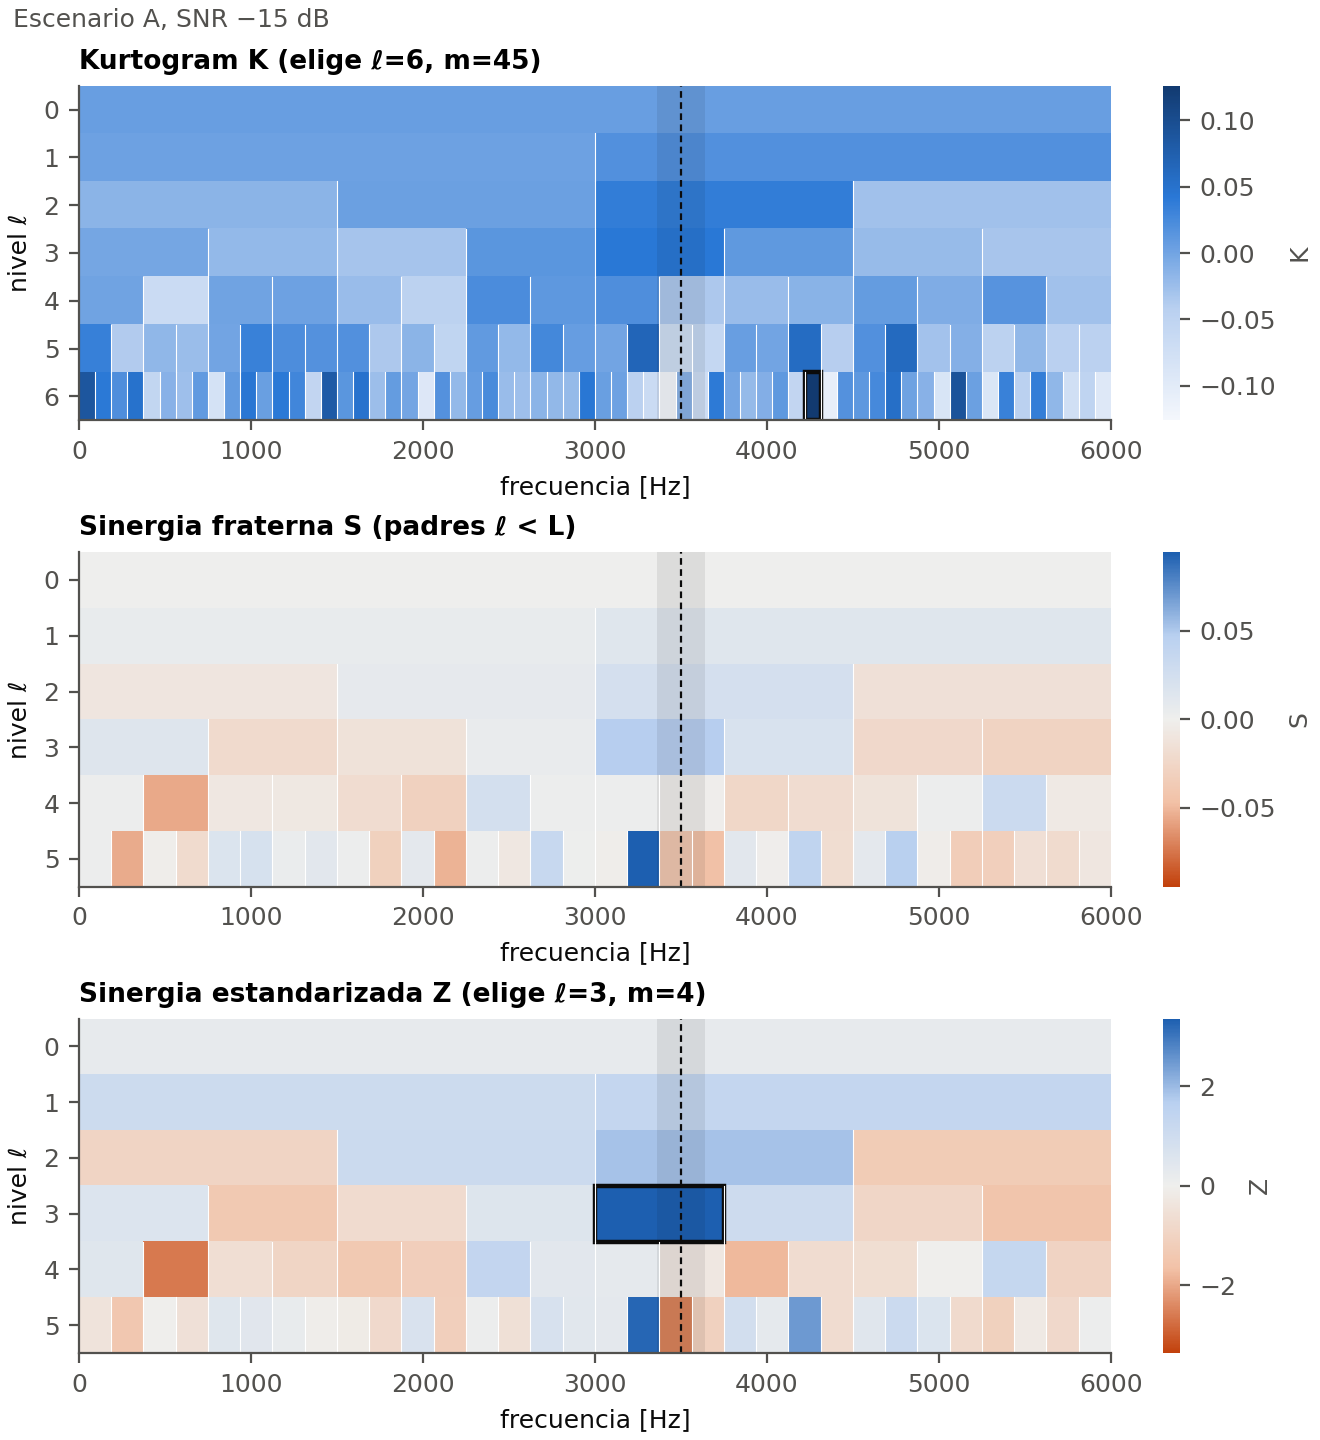
\includegraphics[width=0.84\textwidth]{../fig/mapas_base.png}
\caption{Escenario A, SNR $-15$~dB. El kurtogram elige un nodo del nivel 6 de 94~Hz de ancho, \emph{más angosto que $f_d$}, así que el diagnóstico es imposible. Es el sesgo de profundidad predicho por el Corolario~\ref{cor:sesgo} y la Proposición~\ref{prop:var}. El sinergograma $Z$ elige 3000--3750~Hz, que contiene la resonancia (franja gris), y el SES de esa banda muestra $f_d$ con 8{,}6~dB.}
\label{fig:mapasA}
\end{figure}

\begin{figure}[!htb]
\centering
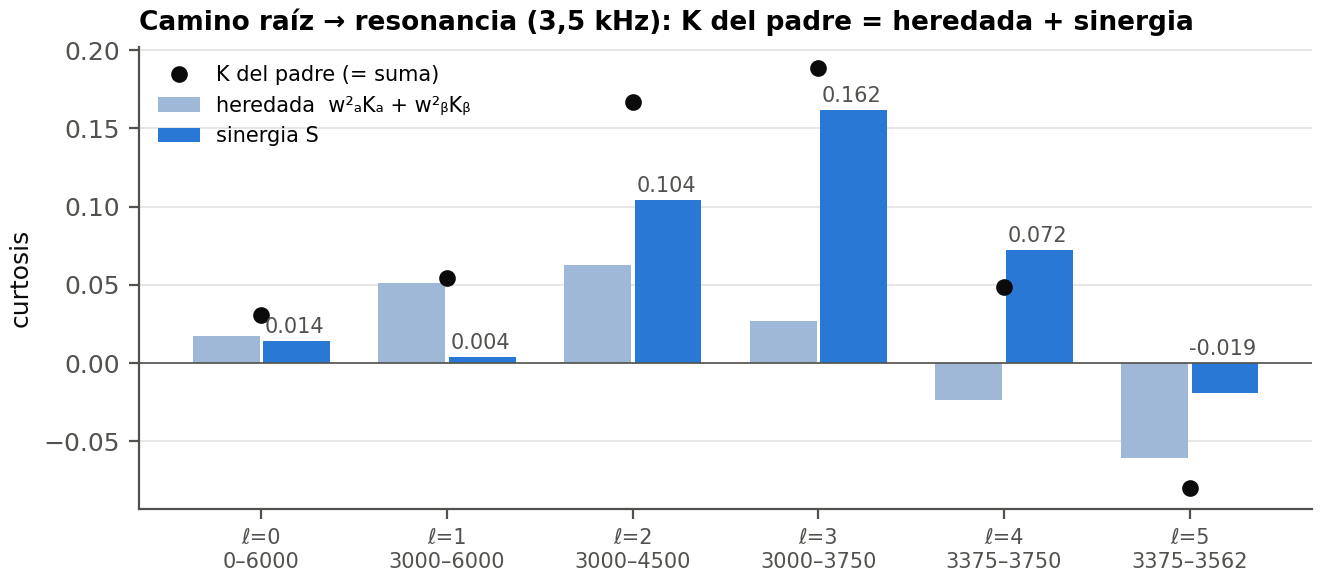
\includegraphics[width=0.8\textwidth]{../fig/herencia.png}
\caption{Identidad \eqref{eq:herencia} a lo largo del camino raíz$\to$resonancia (SNR $-12$~dB). En $\ell=1$ (3--6~kHz, un hijo con la resonancia y otro con ruido) la curtosis del padre es casi toda heredada. En $\ell=2$ y $3$ domina la sinergia: la resonancia ocupa a ambos hijos. En $\ell=4$ la parte heredada ya es negativa y sólo la sinergia sostiene $K$. En $\ell=5$ los hijos (94~Hz) son más angostos que $f_d$ y no pueden contener la modulación: ambas partes son negativas.}
\label{fig:herencia}
\end{figure}

\begin{figure}[!htb]
\centering
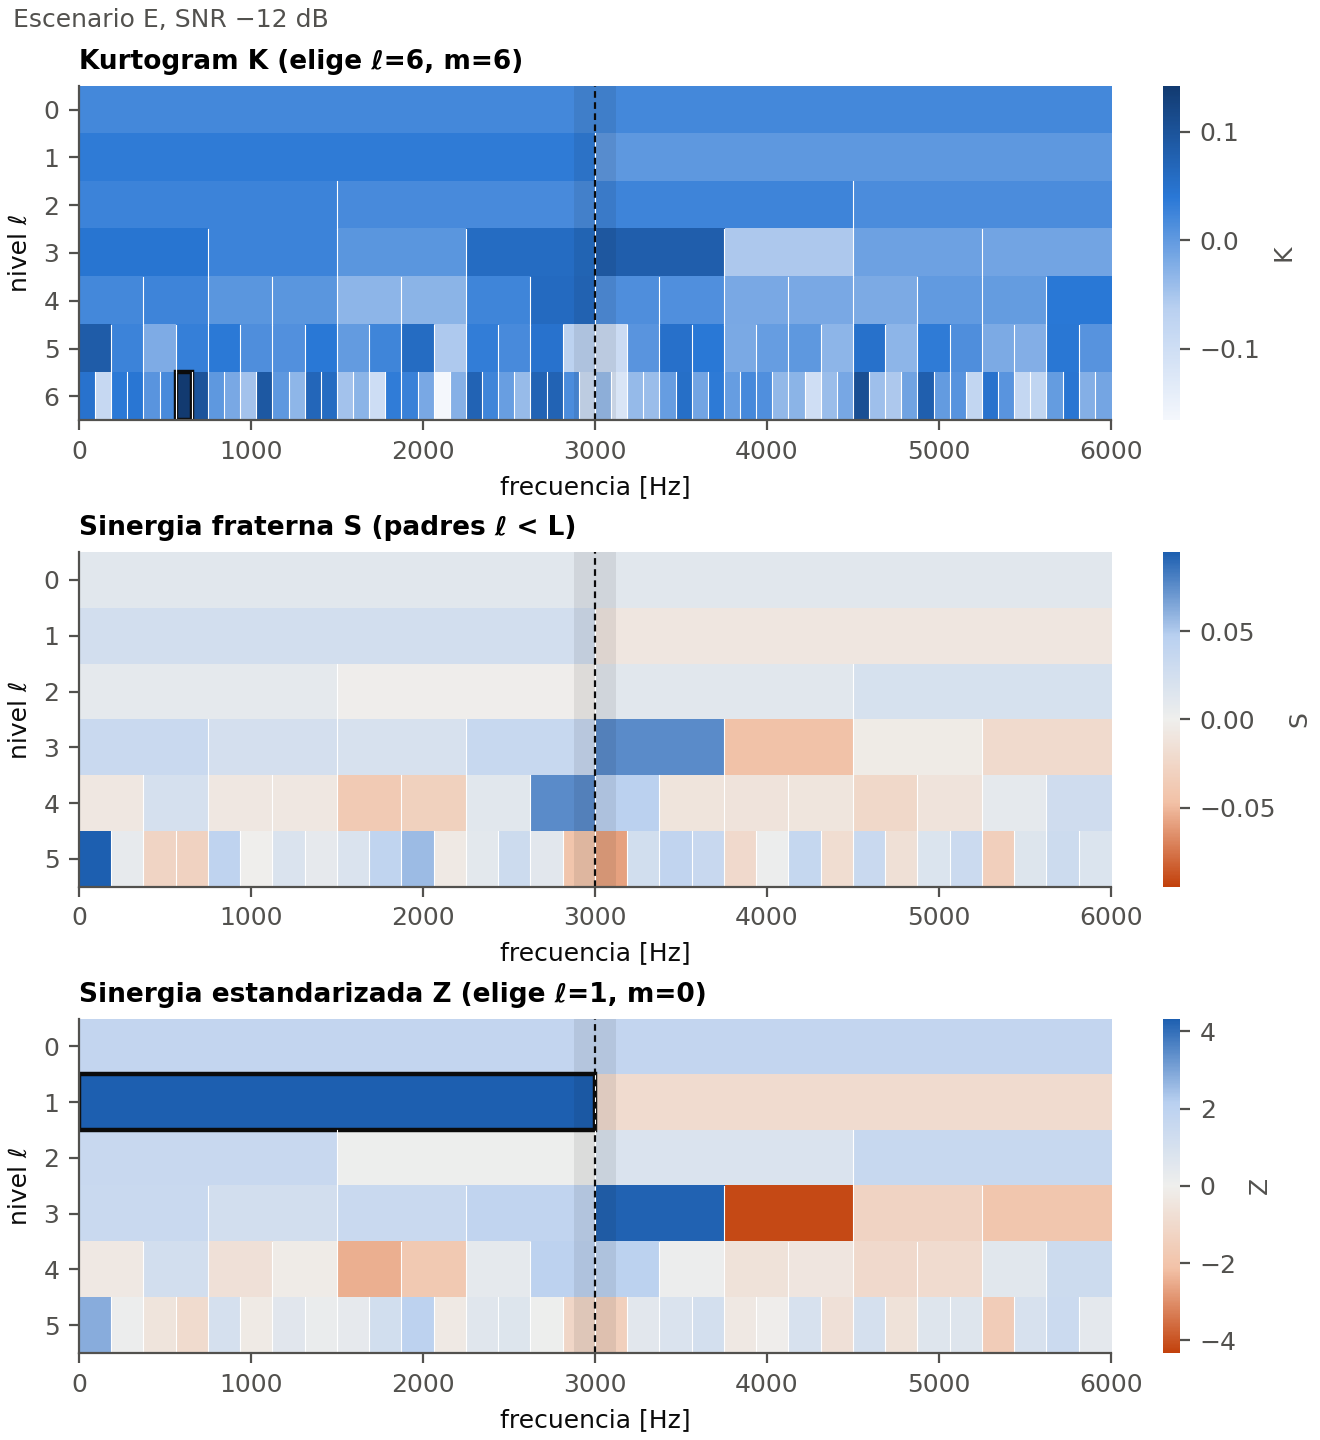
\includegraphics[width=0.84\textwidth]{../fig/mapas_frontera.png}
\caption{Escenario E (resonancia en 3~kHz, sobre una frontera diádica), SNR $-12$~dB. El kurtogram vuelve a caer en un nodo de 94~Hz lejos de la resonancia (562--656~Hz). $Z$ elige 0--3000~Hz, que contiene la mitad inferior de la resonancia, y también marca 3000--3750~Hz, la mitad superior. La sinergia sigue a la resonancia a ambos lados de la frontera, aunque ningún nodo diádico la contenga entera. Esto motiva la idea 6 (sinergia entre primos).}
\label{fig:mapasE}
\end{figure}

\subsection{Monte Carlo en simulación}
\begin{figure}[!htb]
\centering
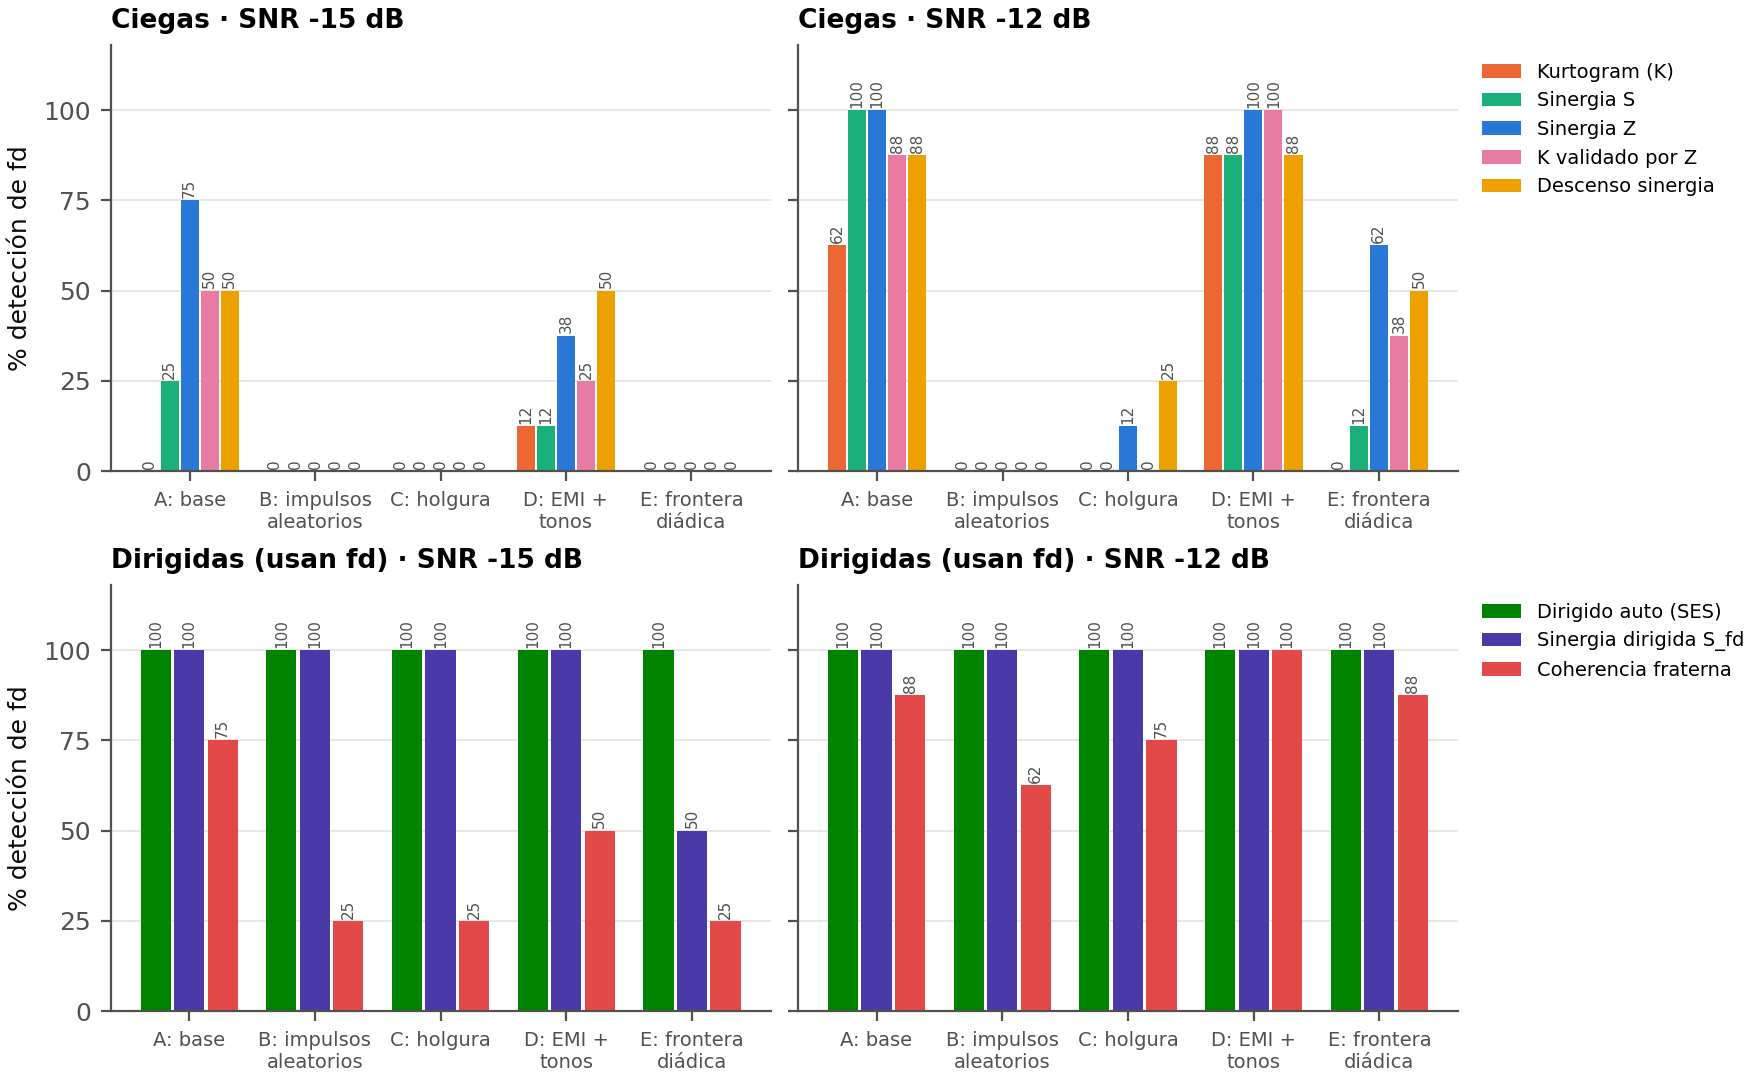
\includegraphics[width=\textwidth]{../fig/montecarlo.png}
\caption{Porcentaje de réplicas en que la banda elegida permite ver $f_d$ (8 réplicas por barra). A $-18$~dB ningún método ciego detecta (no se muestra).}
\label{fig:mc}
\end{figure}

\begin{table}[!htb]
\centering\small
\begin{tabular}{@{}lccccc|ccccc@{}}
\toprule
& \multicolumn{5}{c|}{SNR $-15$ dB} & \multicolumn{5}{c}{SNR $-12$ dB}\\
Método (ciego) & A & B & C & D & E & A & B & C & D & E\\
\midrule
Kurtogram $K$ (clase) & 0 & 0 & 0 & 12 & 0 & 62 & 0 & 0 & 88 & 0\\
Sinergia $S$ & 25 & 0 & 0 & 12 & 0 & \textbf{100} & 0 & 0 & 88 & 12\\
\textbf{Sinergia $Z$} & \textbf{75} & 0 & 0 & 38 & 0 & \textbf{100} & 0 & 12 & \textbf{100} & \textbf{62}\\
Descenso por sinergia & 50 & 0 & 0 & \textbf{50} & 0 & 88 & 0 & \textbf{25} & 88 & 50\\
\bottomrule
\end{tabular}
\caption{Detección (\%) de los métodos ciegos en simulación.}
\label{tab:mc}
\end{table}

\noindent\textbf{Lectura.}
(1) Con ruido gaussiano, EMI y tonos (A, D) y con resonancia en frontera (E), la sinergia estandarizada supera claramente al kurtogram: 75 contra 0\% en A a $-15$~dB y 62 contra 0\% en E a $-12$~dB. Los tonos y la EMI no la engañan, como predice la tabla de interpretación física.
(2) Con impactos que \emph{no} vienen del rodamiento (B aleatorios, C holgura), todos los métodos ciegos fallan, incluida la sinergia. Es la limitación honesta de cualquier criterio de impulsividad y motiva la versión cíclica.
(3) Las métricas dirigidas (fila inferior de la Fig.~\ref{fig:mc}) detectan casi siempre desde $-15$~dB. La sinergia dirigida $S_{f_d}$ empata con el índice dirigido clásico salvo en E a $-15$~dB. La coherencia fraterna normalizada rinde menos. \emph{En simulación no se controló la falsa alarma de los métodos dirigidos}; eso se mide en CWRU.

\subsection{CWRU}
\begin{figure}[!htb]
\centering
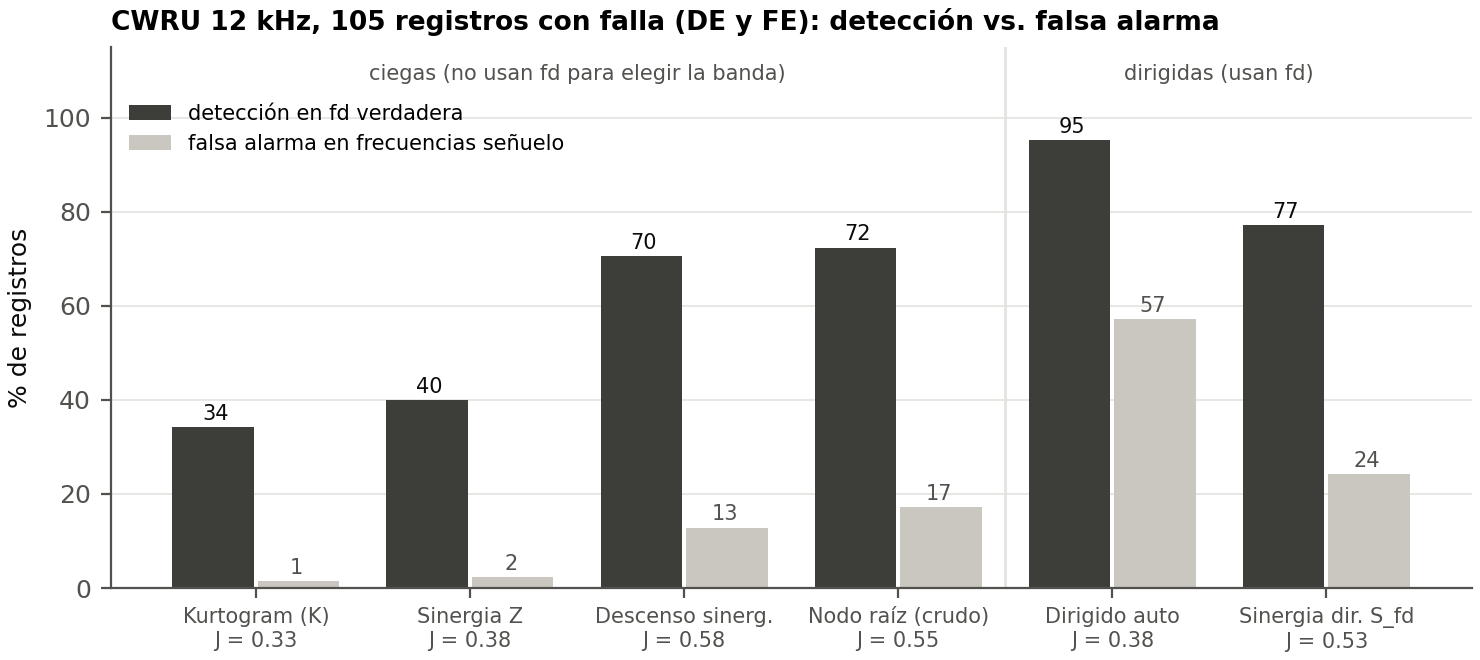
\includegraphics[width=0.95\textwidth]{../fig/cwru_resumen.png}
\caption{Detección en la $f_d$ verdadera frente a detección en frecuencias señuelo (falsa alarma) y $J=$TPR$-$FPR.}
\label{fig:cwru}
\end{figure}

\begin{table}[!htb]
\centering\footnotesize\setlength{\tabcolsep}{4pt}
\begin{tabular}{@{}lccc|ccc|cc|c@{}}
\toprule
& \multicolumn{3}{c|}{Categoría Smith--Randall} & \multicolumn{3}{c|}{Tipo de falla} & \multicolumn{2}{c|}{Sensor} & FA \\
Método & Y (70) & P (17) & N (18) & IR (28) & OR (49) & B (28) & DE (60) & FE (45) & señuelos\\
\midrule
Kurtogram $K$ & 37 & 35 & 22 & 39 & 47 & 7 & 3 & 76 & 1\\
Sinergia $Z$ & 51 & 29 & 6 & 50 & 51 & 11 & 18 & 69 & 2\\
Descenso por sinergia & 93 & 35 & 17 & 89 & 84 & 29 & 72 & 69 & 13\\
Nodo raíz (SES crudo) & 94 & 35 & 22 & 93 & 84 & 32 & 77 & 67 & 17\\
\midrule
Dirigido auto (SES) & 99 & 88 & 89 & 93 & 98 & 93 & 93 & 98 & 57\\
Sinergia dirigida $S_{f_d}$ & 96 & 47 & 33 & 93 & 94 & 32 & 78 & 76 & 24\\
\bottomrule
\end{tabular}
\caption{CWRU 12~kHz: \% de registros con $f_d$ visible, por grupo, y falsa alarma (FA, \%) en señuelos.}
\label{tab:cwru}
\end{table}

\noindent\textbf{Lectura honesta de CWRU.}
\begin{enumerate}[leftmargin=*,itemsep=2pt]
\item \textbf{$Z$ contra el kurtogram:} 40 contra 34\% de detección con la misma falsa alarma (2 y 1\%). En la comparación pareada, $Z$ gana en 10 registros y pierde en 4. La mejora es real pero moderada.
\item \textbf{Ambos pierden contra la envolvente de la señal cruda (72\%).} La causa se ve en la Fig.~\ref{fig:cwru105}: muchos registros DE contienen ráfagas impulsivas \emph{ajenas al rodamiento}, concentradas en bandas angostas (en el registro 105, $K\approx200$ en 5{,}9--6~kHz, junto a Nyquist). El kurtogram las elige y sólo detecta el 3\% de los registros DE. $Z$ también cae en ellas, porque un impulso aislado co-modula a los hermanos (escenario B). Esto es coherente con lo que Smith \& Randall (2015) describen en CWRU: EMI con portadoras de alta frecuencia (armónicos de $\sim$4{,}2~kHz con bandas laterales a $f_r$), armónicos altos del giro atribuibles a holgura y pulsos aparentemente aleatorios en varios registros.
\item \textbf{El descenso por sinergia}, la regla que usa el árbol de forma explícita, detecta el 70\% (43 aciertos donde el kurtogram falla, contra 5 al revés) y tiene menos falsa alarma que la señal cruda (13 contra 17\%). En 65 de 105 registros se detiene en el nivel 1: en CWRU los impactos co-modulan media banda de Nyquist completa, así que la identidad dice ``no dividas más''.
\item \textbf{Métricas dirigidas:} el índice clásico (energía del SES en armónicas de $f_d$, del tipo ICS2/RCC) ``detecta'' el 95\%, pero también el 57\% de los señuelos. Al buscar entre 127 bandas la que tiene más energía en \emph{cualquier} frecuencia, casi siempre encuentra algo: es un problema de comparaciones múltiples. La \textbf{sinergia dirigida} detecta el 77\% con 24\% de falsa alarma y logra el mejor $J$ entre las dirigidas (0{,}53 contra 0{,}38). Es lo que predice la Proposición~\ref{prop:insesgo}: en el espectro cruzado entre hermanos el ruido no genera picos positivos.
\item El registro 282 de clases (Fig.~\ref{fig:cwru282}) es categoría N en Smith \& Randall para el sensor FE con los tres métodos. Ningún método ciego lo diagnostica, y la falta de diagnóstico es consistente con esa referencia.
\end{enumerate}

\begin{figure}[!htb]
\centering
\begin{minipage}[t]{0.495\textwidth}\centering
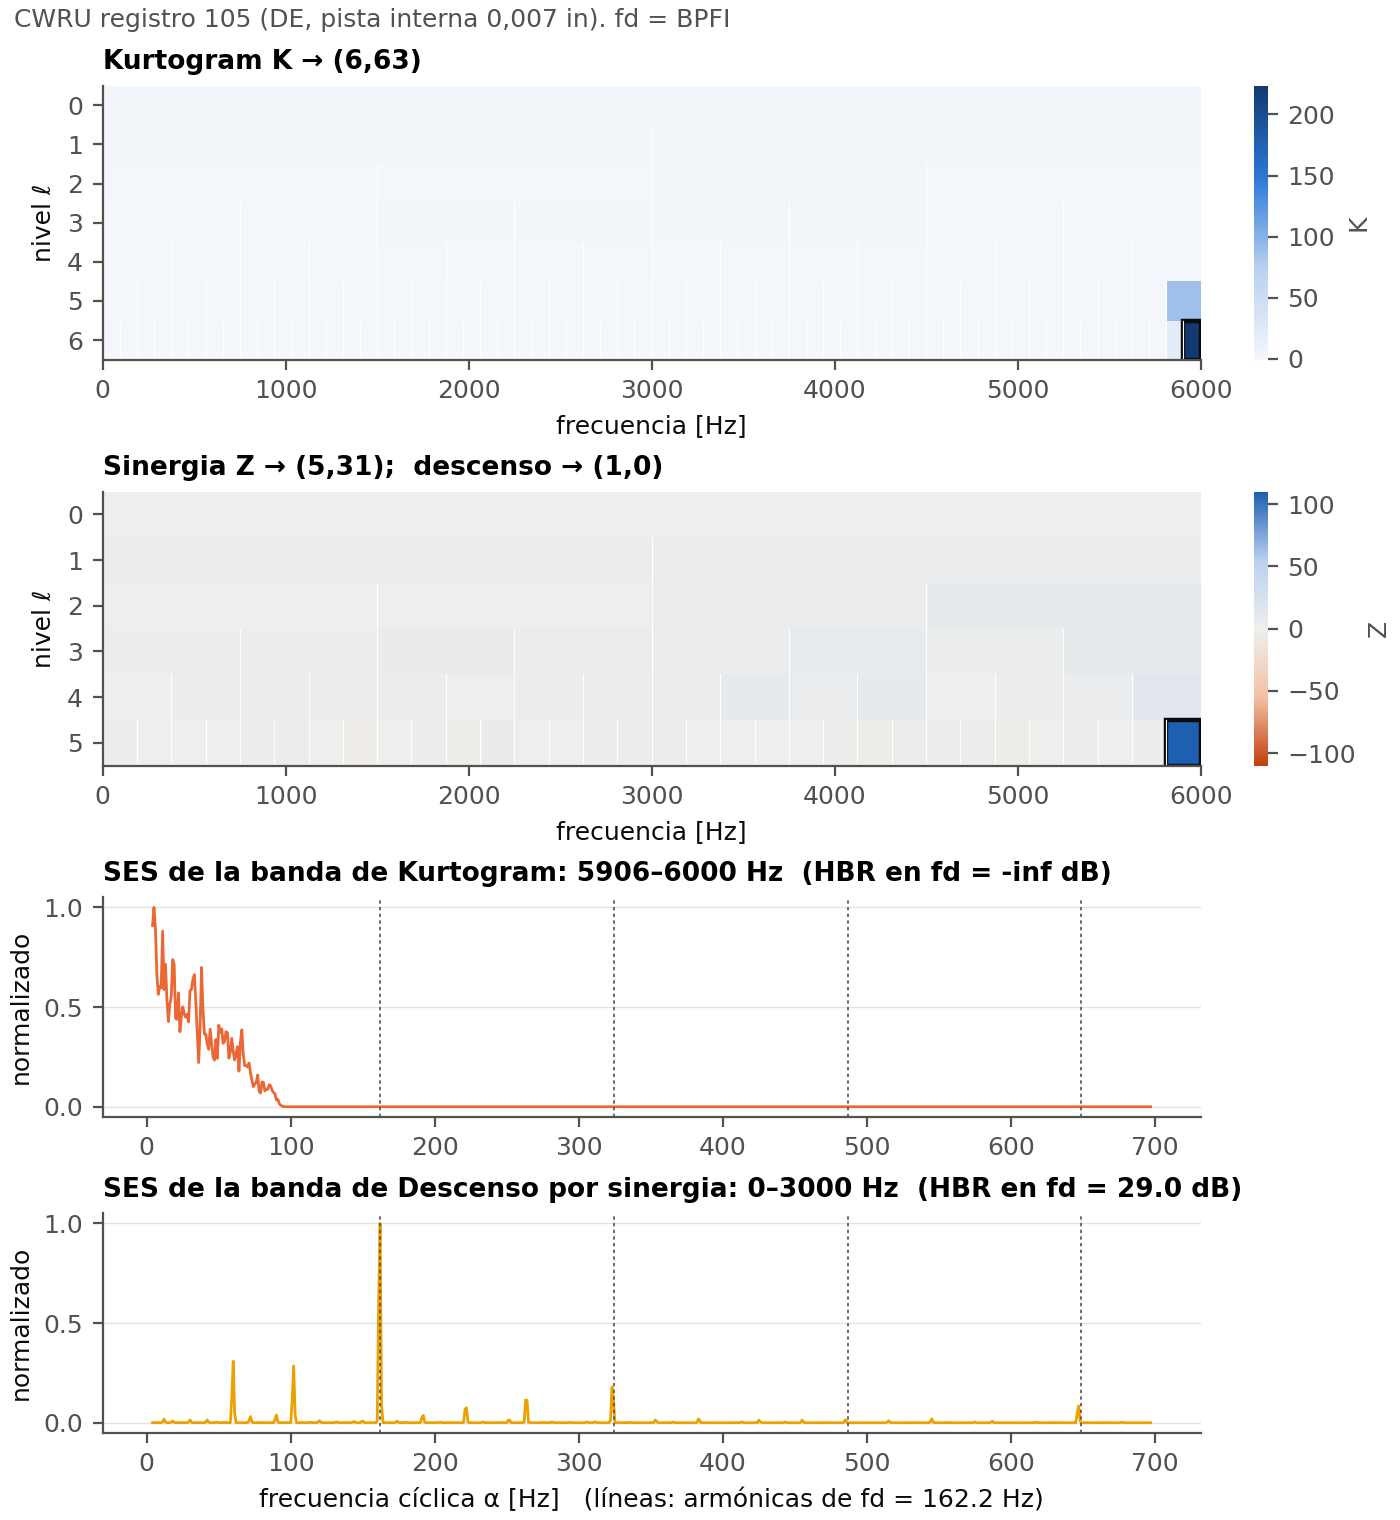
\includegraphics[width=\linewidth]{../fig/cwru_105.png}
\captionof{figure}{Registro 105 (DE, pista interna). El kurtogram elige 5906--6000~Hz por una ráfaga no relacionada con la falla. El descenso por sinergia se detiene en 0--3000~Hz y el SES muestra BPFI con 29~dB.}
\label{fig:cwru105}
\end{minipage}\hfill
\begin{minipage}[t]{0.495\textwidth}\centering
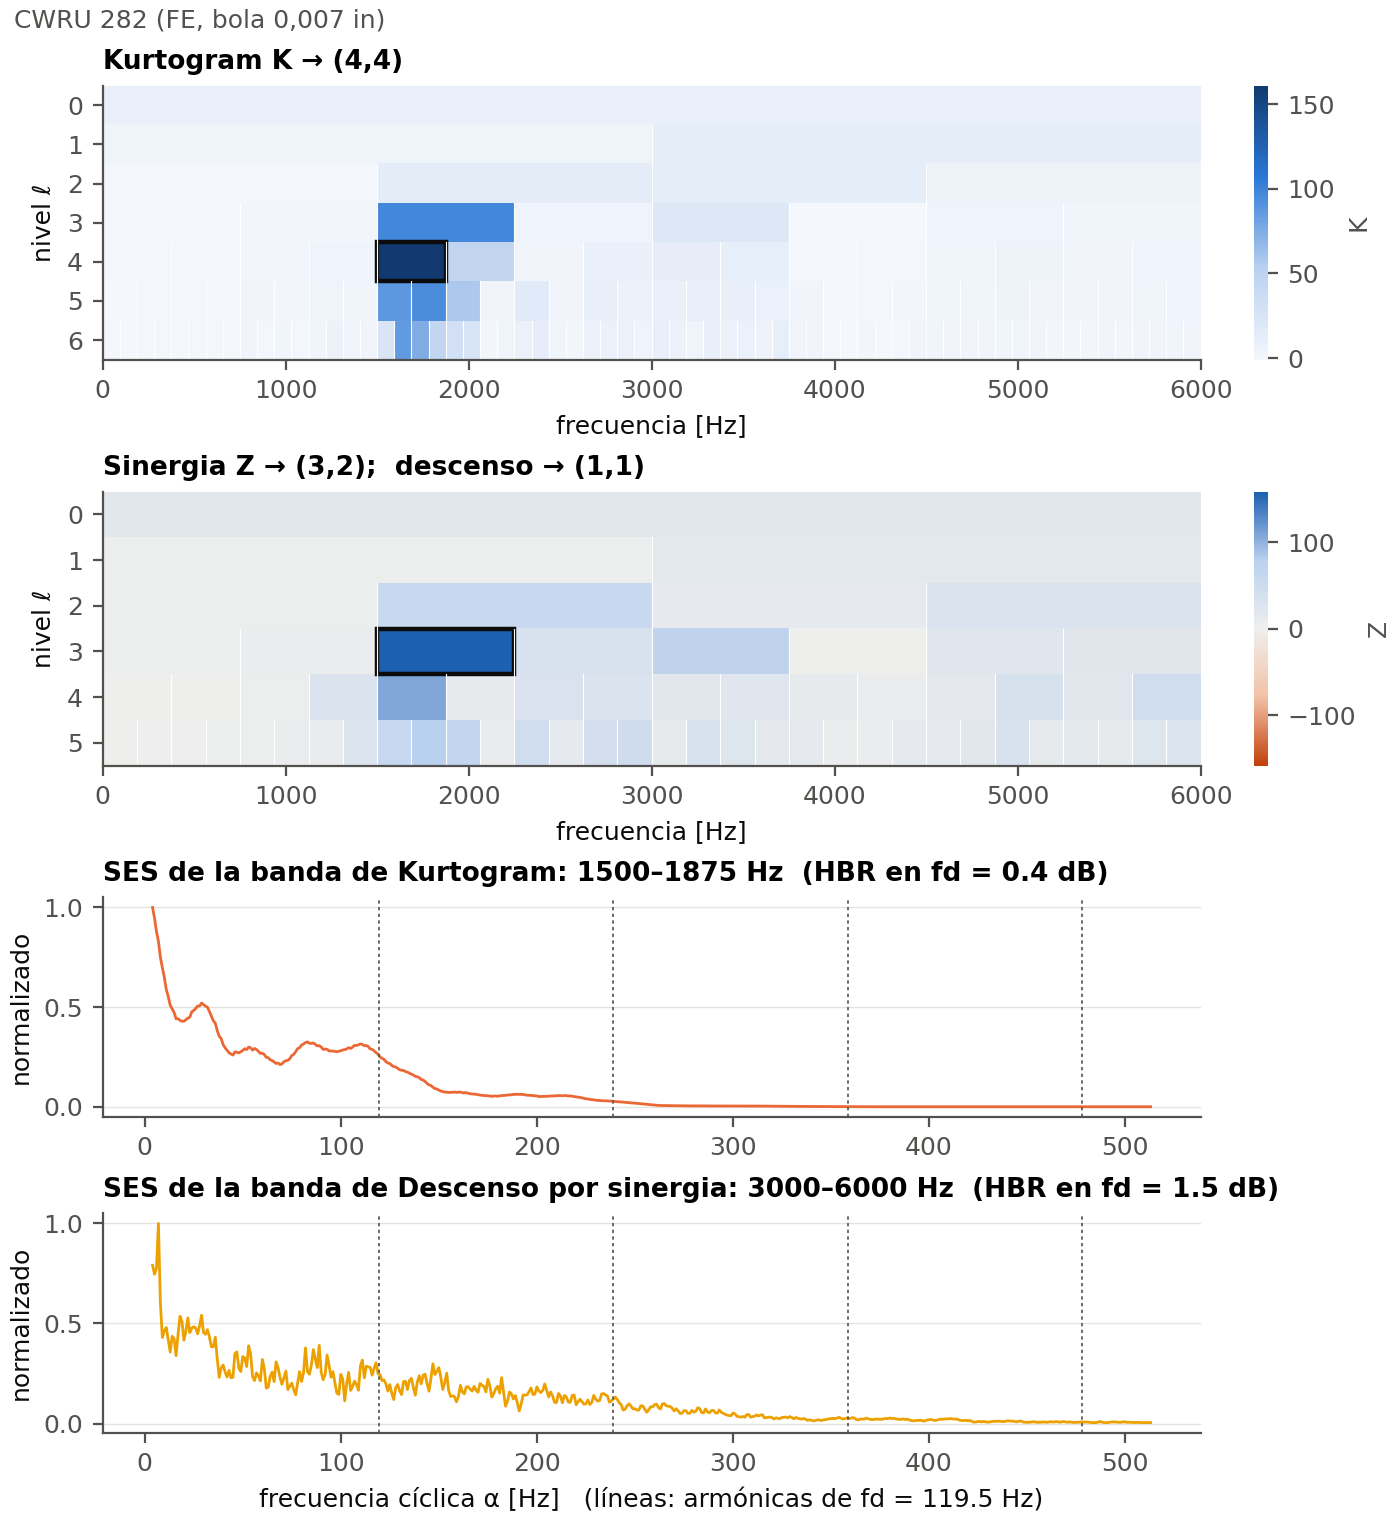
\includegraphics[width=\linewidth]{../fig/cwru_282.png}
\captionof{figure}{Registro 282 (ejemplo de clase, FE, bola 0{,}007 in). $2\,$BSF $=119{,}5$~Hz no aparece con ningún método ciego. Es un registro ``no diagnosticable'' según el benchmark de Smith \& Randall.}
\label{fig:cwru282}
\end{minipage}
\end{figure}

\subsection{Conclusiones}
\begin{enumerate}[leftmargin=*,itemsep=2pt]
\item El árbol MDFD admite una \textbf{identidad exacta} ($K_p=w_a^2K_a+w_b^2K_b+S_p$) que separa la curtosis de un nodo en lo heredado de sus hijos y lo que emerge de su interacción. Es el aporte central: convierte la estructura del árbol en información.
\item La identidad \textbf{explica} el principal defecto del kurtogram: sin sinergia la curtosis se diluye al subir por el árbol, y el ruido de estimación crece como $2^{\ell/2}$ al bajar. Por eso el $\arg\max$ resbala hacia hojas inútiles: a $-15$~dB el kurtogram detectó 0\% en 4 de los 5 escenarios.
\item La \textbf{sinergia estandarizada} $Z$ corrige ese sesgo en ruido gaussiano, EMI, tonos y resonancias en frontera diádica. En CWRU mejora al kurtogram de forma moderada.
\item Las dos variantes que usan el árbol de forma más explícita dieron los mejores compromisos detección/falsa alarma de sus familias en CWRU: el \textbf{descenso por sinergia} ($J=0{,}58$) y la \textbf{sinergia dirigida} ($J=0{,}53$).
\item Ninguna métrica de impulsividad ciega distingue impactos del rodamiento de impactos ajenos. La vía natural es la \textbf{sinergia cíclica ciega} (idea 10), que busca en $s_p(\alpha)$ un peine armónico sin conocer $f_d$.
\end{enumerate}


%==========================================================================
\section{¿Es nuevo? Relación con la literatura}
%==========================================================================
\begin{itemize}[leftmargin=*]
\item \textbf{Kurtogram / fast kurtogram} (Antoni 2006, 2007): evalúa $K$ nodo por nodo. Aquí se usa su árbol, pero se agrega la relación padre--hijos.
\item \textbf{Infogram} (Antoni 2016) y sus variantes: combinan negentropía de SE y SES por nodo, sin relación entre nodos.
\item \textbf{Mapas de correlación/dependencia entre bins del espectrograma} (grupo de Wrocław: Nowicki, Hebda-Sobkowicz, Wodecki, Zimroz; 2021--2025). Es lo más cercano: correlacionan sub-señales de \emph{bins} vecinos de un espectrograma plano para encontrar la banda informativa. No usan un árbol, no descomponen la curtosis ni tienen la identidad \eqref{eq:herencia}, la nula por surrogados fraternos, la descomposición cíclica \eqref{eq:sespectro} ni el resultado de insesgo.
\item \textbf{Best-basis / poda de wavelet packets} (Coifman--Wickerhauser 1992) y \textbf{árboles ocultos de Markov} (Crouse, Nowak y Baraniuk 1998): usan relaciones padre--hijo para \emph{elegir bases} o \emph{modelar persistencia} de coeficientes, pero no para descomponer la curtosis ni para seleccionar bandas de demodulación.
\item \textbf{Indicadores dirigidos} (ICS2, RCC, log-cycligram; Smith \emph{et al.} 2019): el índice ``Dirigido auto (SES)'' usado aquí como referencia es de esa familia.
\item \textbf{Espectros de envolvente de producto} (PESOgram, Chen \emph{et al.} 2023; EGOgram, Wang \emph{et al.} 2026). Combinan multiplicativamente los espectros de envolvente de varias bandas; el EGOgram usa dos bandas ``fuertemente correlacionadas''. Es el pariente más cercano del espectro de sinergia $s_p(\alpha)$. La diferencia: $s_p$ es un espectro \emph{cruzado} con una justificación exacta (su integral es $S^{\mathrm{cov}}$ y el ruido tiene media cero, Prop.~\ref{prop:insesgo}).
\end{itemize}
\textbf{Búsqueda sistemática en Scopus y Web of Science} (23-09-2026, acceso PUCV; detalle en \texttt{busqueda\_bibliografica.md}). El campo de la selección de banda para rodamientos tiene 601 documentos en Scopus y 646 en WoS, con unos 50--65 por año. Las búsquedas de descomposición o herencia de la curtosis por sub-bandas, co-curtosis entre bandas, métricas padre--hijo o de hermanos en el árbol, espectro cruzado de envolventes cuadráticas entre bandas y selección de banda con surrogados o pruebas de hipótesis \textbf{no devolvieron ningún trabajo equivalente} en ninguna de las dos bases. Los trabajos más cercanos son los mapas de dependencia (Wrocław) y los espectros de envolvente de producto. Por eso el aporte se plantea como: (i) la identidad exacta y sus consecuencias, (ii) la nula con surrogados fraternos y (iii) la base teórica del espectro cruzado entre hermanos.

%==========================================================================
\section{Limitaciones y trabajo futuro}
%==========================================================================
\begin{enumerate}[leftmargin=*]
\item La sinergia ciega detecta \emph{co-impulsividad}, no ``falla de rodamiento''. Igual que el kurtogram, puede ser engañada por impactos aleatorios o periódicos que no provienen del rodamiento (escenarios B y C). La salida es la versión cíclica, idealmente ciega (idea 10).
\item Un peine de armónicos de línea con fases fijas puede producir co-modulación a 60~Hz (batidos) y con ello $S\ne0$. Es detectable en $s_p(\alpha)$ a $\alpha=60$~Hz.
\item Si la resonancia cae completamente dentro de un solo hijo, la sinergia del padre es baja aunque el padre contenga la resonancia. Por diseño, la métrica prefiere la banda más ancha que sigue siendo ``indivisible''.
\item Los surrogados cuestan $R$ evaluaciones extra por padre ($\sim$6~s por registro de 10~s con $L=6$, $R=12$, en un portátil). El costo es aceptable, pero se puede reducir con la varianza asintótica.
\item Pendiente: sinergia entre primos (resonancias partidas por fronteras de niveles superiores), árbol 1/3-binario y validación en Paderborn/XJTU-SY.
\end{enumerate}

\section*{Reproducibilidad}
El código (\texttt{mdfd\_sinergia.py}, \texttt{simulador.py}) y el notebook \texttt{sinergia\_fraterna.ipynb} reproducen todas las figuras. Los datos CWRU provienen del Bearing Data Center de Case Western Reserve University. Las categorías de referencia son las de Smith \& Randall (2015), Tablas B2 y B4.

\begin{thebibliography}{9}\small
\bibitem{antoni2007} J.~Antoni, ``Fast computation of the kurtogram for the detection of transient faults,'' \emph{MSSP} 21 (2007) 108--124.
\bibitem{antoni2016} J.~Antoni, ``The infogram: Entropic evidence of the signature of repetitive transients,'' \emph{MSSP} 74 (2016) 73--94.
\bibitem{smith2015} W.A.~Smith, R.B.~Randall, ``Rolling element bearing diagnostics using the Case Western Reserve University data: A benchmark study,'' \emph{MSSP} 64--65 (2015) 100--131.
\bibitem{smith2016} W.A.~Smith, Z.~Fan, Z.~Peng, H.~Li, R.B.~Randall, ``Optimised spectral kurtosis for bearing diagnostics under electromagnetic interference,'' \emph{MSSP} 75 (2016) 371--394.
\bibitem{smith2019} W.A.~Smith \emph{et al.}, ``Optimal demodulation-band selection for envelope-based diagnostics: A comparative study of traditional and novel tools,'' \emph{MSSP} 134 (2019) 106303.
\bibitem{wroclaw} ``Robust correlation measures for informative frequency band selection in heavy-tailed signals,'' arXiv:2502.11192 (2025), y referencias ahí (Nowicki \emph{et al.} 2021; Hebda-Sobkowicz \emph{et al.} 2021).
\bibitem{coifman} R.R.~Coifman, M.V.~Wickerhauser, ``Entropy-based algorithms for best basis selection,'' \emph{IEEE Trans.\ Inf.\ Theory} 38 (1992) 713--718.
\bibitem{crouse} M.S.~Crouse, R.D.~Nowak, R.G.~Baraniuk, ``Wavelet-based statistical signal processing using hidden Markov models,'' \emph{IEEE Trans.\ Signal Process.} 46 (1998) 886--902.
\bibitem{pes} B.~Chen \emph{et al.}, ``Product envelope spectrum optimization-gram: An enhanced envelope analysis for rolling bearing fault diagnosis,'' \emph{MSSP} (2023) 110270.
\bibitem{ego} X.~Wang \emph{et al.}, ``EGOgram: an adaptive frequency band division and dual band synergistic enhancement method for fault diagnosis of wind turbine yaw bearings,'' \emph{Meas.\ Sci.\ Technol.} 37 (2026) 306110.
\bibitem{nowicki} J.~Nowicki, J.~Hebda-Sobkowicz, R.~Zimroz \emph{et al.}, ``Dependency measures for the diagnosis of local faults in application to the heavy-tailed vibration signal,'' \emph{Applied Acoustics} (2021) 107974.
\bibitem{randall2011} R.B.~Randall, J.~Antoni, ``Rolling element bearing diagnostics---A tutorial,'' \emph{MSSP} 25 (2011) 485--520.
\end{thebibliography}
\end{document}
